% \documentclass[14pt]{extarticle}
\documentclass[bibliography=totocnumbered]{scrartcl}
% \usepackage[english]{babel}
\usepackage[russian]{babel}
\usepackage[utf8x]{inputenc}
\usepackage{amsmath}
\usepackage{graphicx}
\usepackage[colorinlistoftodos]{todonotes}
\usepackage{amssymb}
\usepackage{amsmath}
\usepackage{graphicx}
\usepackage[margin=.8in]{geometry}
\usepackage{listings}
\usepackage[section]{placeins}
\begin{document}

\begin{titlepage}
\newgeometry{margin=2cm}
\newcommand{\HRule}{\rule{\linewidth}{0.5mm}}
\center
\textsc {
\footnotesize{
минобрнауки россии\\
федеральное государственное бюджетное образовательное учреждение\\
высшего профессионального образования}\\
\large{Воронежский государственный университет}
}\\[1.0cm]
\textsc{\largeФакультет компьютерных наук}\\
\textsc{\footnotesizeКафедра информационных технологий}\\[1.0cm] 
\textsc{\Large Эссе}\\[0.5cm]
\HRule \\[0.4cm]
{ \huge \bfseries Системная инженерия на примере системы «Газовый котёл»}\\[0.4cm] % Title of your document
\HRule \\[1.5cm]


\begin{flushleft} \large
% \emph{Зав. кафедрой:} Э.К. \textsc{Алгазинов}, д. ф-м н., проф.\\
\emph{Студент:} А.А. \textsc{Валиков} \\
% \emph{Руководитель:} А.В. \textsc{Стромов}, к. ф-м н. % Supervisor's Name
\end{flushleft}

\vfill
\begin{center}
Воронеж 2018
\end{center}
\end{titlepage}

\tableofcontents

\newpage

\section{Введение}

\subsection{Функциональные требования стейкхолдеров}

\paragraph{Пользователи}
\begin{itemize}
  \item Низкие расходы (цена котла, потребление газа, обслуживание)
\end{itemize}

\paragraph{Комиссия по сертификации}
\begin{itemize}
  \item Безопасность (например, газовый затвор имеет дублированную схему)
\end{itemize}

\paragraph{Производитель}
\begin{itemize}
  \item Высокий спрос
  \item Минимальные затраты на ресурсы и рабочую силу
\end{itemize}
Основная функция -- \textbf{нагревать воду и перемещать её по системе отопления}

\subsection{Конструкционные ограничения архитектуры}
Котёл представляет из себя сложную систему, опишем его в общем, с некоторыми допущениями.

\begin{figure}[htp]
  \centering
  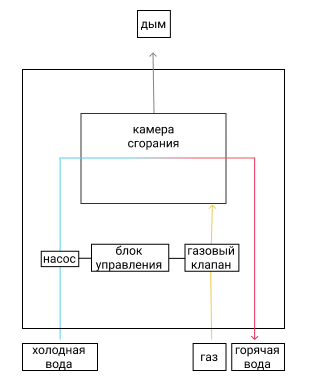
\includegraphics[scale=1.00]{arch.png}
\end{figure}

\subsection{Описываемая система как холон в иерархии}
Рассмотрим какое место может занять рассматриваемая система как холон в иерархии других холонов -- холархии.
\begin{figure}
  \centering 
\includegraphics[scale=0.5]{hol.png}
\end{figure}
\subsection{Системы: целевая, обеспечивающая, в эксплуатационной среде}

\paragraph{Целевая система}
Целевой системой как нетрудно догадаться является собственно газовый котёл.

\paragraph{Обеспечивающая система}
\begin{itemize}
  \item Сырьё и компоненты для сборки
  \item Здание завода
  \item Оборудование
  \item Проекты котлов
  \item Персонал
\end{itemize}

\paragraph{Система в эксплуатационной среде}
По каждому типу ресурсов можно выделить соответствующую систему, необходимую при эксплуатации целевой системы:

\begin{itemize}
  \item
    \textbf{Электроэнергия}
    \begin{itemize}
      \item Производители электроэнергии: АЭС, ГЭС, ТЭС и другие
      \item Трансформаторы: повышающие (для передачи на большие расстояния) и понижающие (для доставки конечному потребителю)   
      \item Коммуникации: внутридомовая проводка, провода в гордской черте, ЛЭП
    \end{itemize}
  
  \item
    \textbf{Газ}
    \begin{itemize}
      \item Организации, занимающиеся геологоразведкой
      \item Бурение и добыча
      \item Центры контроля состояния
      \item Транспортировка: как правило трубопровод, ближе к потребителю могут использоваться баллоны
    \end{itemize}
  
  \item
    \textbf{Вода для системы отопления}
    \begin{itemize}
      \item Получение: городское водохранилище, скважина
      \item Транспортировка: магистральные трубы, водопровод внутри дома
      \item Узлы фильтрации
      \item Узлы запорной арматуры: краны, вентили
    \end{itemize}
  
  \item
    \textbf{Отведение дыма}
    \begin{itemize}
      \item Узлы примыкания к дымоходу
      \item Трубы дымохода: общедомовой дымоход или собственный
    \end{itemize}
\end{itemize}

Опишем также людей, которым предстоит взаимодействовать с системой:
\begin{itemize}
  \item Жители дома или квартиры.
  \item Сервисная служба.
\end{itemize}

\section{Жизненный цикл системы согласно V-диаграмме}

\subsection{Определение требований}
На данной стадии происходит сбор и анализ требований к будущей
игре, которые формулируются стейкхолдерами. Требования могут касаться:
\begin{itemize}
  \item Мощности котла
  \item Наличия функции нагрева горячей воды
  \item Стоимости исходных компонентов и сложности сборки
  \item Устойчивость к перепадам ресурсов (напяжение в сети и давление газа)
\end{itemize}

\subsection{Архитектурное проектирование}
Создаётся дизайн котла, согласно требованиям, определённым на предыдущем этапе, решается какие узлы нужны в системе (если котёл умеет греть горячую воду, нужен второй теплообменник). Создаются принципиальные схемы взаимодействия между узлами

\subsection{Рабочее проектирование}
Теперь, когда решено какие именно ключевые узлы будут в системе, необходимо спроектировать в САПР 3D модель а также указать все проектируемые коммуникации и взаимодействия между узлами. Специалистам предстоит спроектировать отдельные узлы, например плату управления, насос, газовый клапан. Для всех узлов также будут пройдены этапы разработки V-диаграммы.

\subsection{Изготовление}
На этом этапе воплощаются проекты узлов:
\begin{itemize}
  \item Станками или рабочими на плате управления вытравливаются токопроводящие дорожки, припаиваются электронные компоненты
  \item Сварщиками создаётся теплообменник и узлы подводки
  \item В отделе формовки из пластика отливаются корпуса для различных частей
\end{itemize}
Каждый созданный компонент проходит тестирование на соответствие заявленным функциям

\subsection{Интеграция}
Сборщиками отельные узлы собираются в единое устройство: плата помещается в корпус и соединяется с остальными узлами, размещается теплообменник и соединяется с подводкой воды

\subsection{Приём в эксплуатацию и эксплуатация}
Окончательное тестирование всего котла, можно привести несколько примеров:

\begin{itemize}
  \item Соответствует соотношение между отдаваемым теплом и потребляемым газом заяявленному
  \item Как ведёт себя котёл при скачках напряжения
  \item Сколько времени уходит нагрев некоторой площади
  \item И многие другие
\end{itemize}
Если все тесты пройдены, котёл может быть передан в реализацию. Иначе, выясняют почему некоторый параметр не в норме, какие при этом задействованы узлы. В зависимости от серьёзности ошибки, разработка может вернуться либо к рабочему проектированию (если ошибка невелика) либо к архитектурному или даже к сбору требований.

\section{Практики системной инженерии}
В стандарте ISO 15288:2008 указаны 25 обязательных практик системной инженерии. Опишем технические практики, так как именно они непосредственно связаны с целевой системой.

\subsection{Сбор требований}
От всех стейкхолдеров собираются требования к будущему котлу. В случае в коммисией по сертификации это сертификационные документы. Для потребителей это может быть современный дизайн, компактный размер, маленькая или большая мощность (в зависимости от того, на какую ценовую категорию расчитано устройство). Производитель же хочет, чтобы сборка была наименее трудозатратная и вкючала насколько возможно дешёвые компоненты.

\subsection{Анализ требований}
Требования сводятся в один список и пересматриваются: какие-то могут быть исключены из-за несовместимости друг с другом, другие -- нуждаться в уточнении.

\subsection{Архитектурный дизайн}
Эта практика объединяет в себе этапы «Архитектурное проектирование» и «Рабочее проектирование» V-диаграммы. То есть здесь проектировщик с привлечением различных программных комплексов (редактор UML диграмм, САПР) создаёт сначала общую, концептуальную модель будущего котла. Затем узкие специалисты (по электронике, гидравлике и другие) занимаются проектированием конкретных компонентов системы.

\subsection{Изготовление}
Здесь полностью повторяется этап «Изготовление». То есть проекты воплощаются в реальности, тестируются и, если выявляются ошибки, отправляются на доработку.

\subsection{Интеграция}
То же, что и «Интеграция» в V-диаграмме, -- сборка компонентов.

\subsection{Проверка всей системы}
На этом этапе проводится интеграционное тестирование с целью увидеть как работает система в сборе и если что-то не так, внести коррективы в проект. Здесь же происходит внешний контроль государственной службой сертификации.

\subsection{Переход к эксплуатации}
На заводе собираются стенды для тестирования. Например, холодильная камера с помещёнными внутри радиаторами, для симуляции остывающего дома. Также для проверки UI/UX показателей котёл может быть отправлен в магазины, где клиенты смогут оценить удобство взаимодействия, а магазины отправят собранные данные на завод.

\subsection{Валидация}
Собранная обратная связь изучается и на основе неё составляется список доработок, после чего вносятся коррективы в проект.

\subsection{Эксплуатация}
Котёл упаковывается и доставляется в магазин, чтобы быть проданным покупателям. Отдел маркетинга в сотрудничестве с магазинами может провести рекламную кампанию по привлечению покупателей. После приобретения покупателем, специальная служба устанавливает котёл. 

\subsection{Обслуживание}

\paragraph{Со строны производителя}
Производитель представляет возможность задать вопрос (посредством горячей линии или формы на сайте). Даётся гарантия на определённый срок (при условии соблюдения условий эксплуатации)

\paragraph{Со стороны сервисной службы}
Поставщик газа обязывает пользователей производить ежегодное техобслуживание в фирмах, имеющих лицензию на таку. деятельность. Обычно эти работы входят очистка горелки, проверка давления в системе и другие. 

\subsection{Вывод из эксплуатации}
Опять-таки, разделим эту практику на стороны:

\paragraph{Производитель}
Оценивая ситуацию на рынке и прошедшее с момента вывода модели котла на рынок время, производитель принимает решение о снятии её с производства, а ещё через некоторое время и о прекращении возможности официального ремонта существующих котлов этой модели. При этом проектные наработки и новшества этой модели могут в том или ином виде войти в проекты для будущик котлов.

\paragraph{Пользователь}
Через время, опеределённое производителем, котёл рекомендуется заменить. После этого он может быть сдан в пункт по переработки бытовой техники, при этом большая часть компонентов может быть вторично использована в промышленности.
\end{document}